\documentclass[ignorenonframetext,]{beamer}
\usetheme{Madrid}
\usecolortheme{crane}
\usepackage{amssymb,amsmath}
\usepackage{ifxetex,ifluatex}
\usepackage{fixltx2e} % provides \textsubscript
\ifxetex
  \usepackage{fontspec,xltxtra,xunicode}
  \defaultfontfeatures{Mapping=tex-text,Scale=MatchLowercase}
\else
  \ifluatex
    \usepackage{fontspec}
    \defaultfontfeatures{Mapping=tex-text,Scale=MatchLowercase}
  \else
    \usepackage[utf8]{inputenc}
  \fi
\fi
\usepackage{listings}
\usepackage{caption}
\usepackage{graphicx}
\makeatletter
\def\ScaleIfNeeded{%
  \ifdim\Gin@nat@width>\linewidth
    \linewidth
  \else
    \Gin@nat@width
  \fi
}

\makeatother
% \let\Oldincludegraphics\includegraphics
% \renewcommand{\includegraphics}[2][]{\Oldincludegraphics[width=\ScaleIfNeeded]{#2}}

% Comment these out if you don't want a slide with just the
% part/section/subsection/subsubsection title:
\AtBeginPart{
  \let\insertpartnumber\relax
  \let\partname\relax
  \frame{\partpage}
}
\AtBeginSection{
  \let\insertsectionnumber\relax
  \let\sectionname\relax
  \frame{\sectionpage}
}
\AtBeginSubsection{
  \let\insertsubsectionnumber\relax
  \let\subsectionname\relax
  \frame{\subsectionpage}
}

\setlength{\parindent}{0pt}
\setlength{\parskip}{6pt plus 2pt minus 1pt}
\setlength{\emergencystretch}{3em}  % prevent overfull lines
\setcounter{secnumdepth}{0}
\parindent=20pt
\parskip=8pt

\usepackage{ccfonts,eulervm} 
\usepackage[T1]{fontenc}
\usepackage{epigraph}
\usepackage{amsmath}
\usepackage{amsfonts}
\usepackage{amssymb}
\usepackage{fancyhdr}
\usepackage[activeacute, spanish]{babel}
\usepackage{cancel}
\usepackage[utf8]{inputenc}
\usepackage{algorithm}
\usepackage{algpseudocode}
\usepackage{afterpage}
\usepackage{url}
\usepackage{fancyhdr}

\parindent 0em
\algrenewcommand{\algorithmiccomment}[1]{//\textit{#1} }

\renewcommand{\footrulewidth}{0.4pt}
\newcommand{\hblacksquare}{\hfill \blacksquare}

\lstset{basicstyle=\footnotesize}

\title{Malware para Android}
\author{Darago, Sackmann, Stricker}
\date{\today}

\begin{document}
\frame{\titlepage}

% \begin{frame}
% \tableofcontents[hideallsubsections]
% \end{frame}

\section{Primera parte: robando fotos}

\begin{frame}\frametitle{Mandar las fotos}
\begin{itemize}[<+->]
\itemsep1pt\parskip0pt\parsep0pt
	\item Una vez que tenemos las fotos... ¿cómo las mandamos? \\
	\item Varias opciones:
	\begin{itemize}[<+->]
		\item Mail
		\item MMS
		\item Scp
		\item Post
	\end{itemize}
\end{itemize}

\end{frame}

\begin{frame}\frametitle{¿Quién recibe las fotos?}
	\begin{itemize}[<+->]
		\item Ok, buenísimo, ya sabemos que vamos a mandar las fotos por post.... ¿a dónde?
		\item Levantamos un servidor apache en lo de Juli, para recibir las fotos.
		\item ¡Buenííísimo!. Vamos a probarlo:
	\end{itemize}
\end{frame}

\begin{frame}\frametitle{¡Anduvo!}
	\begin{figure}[htbp]
		\centering
		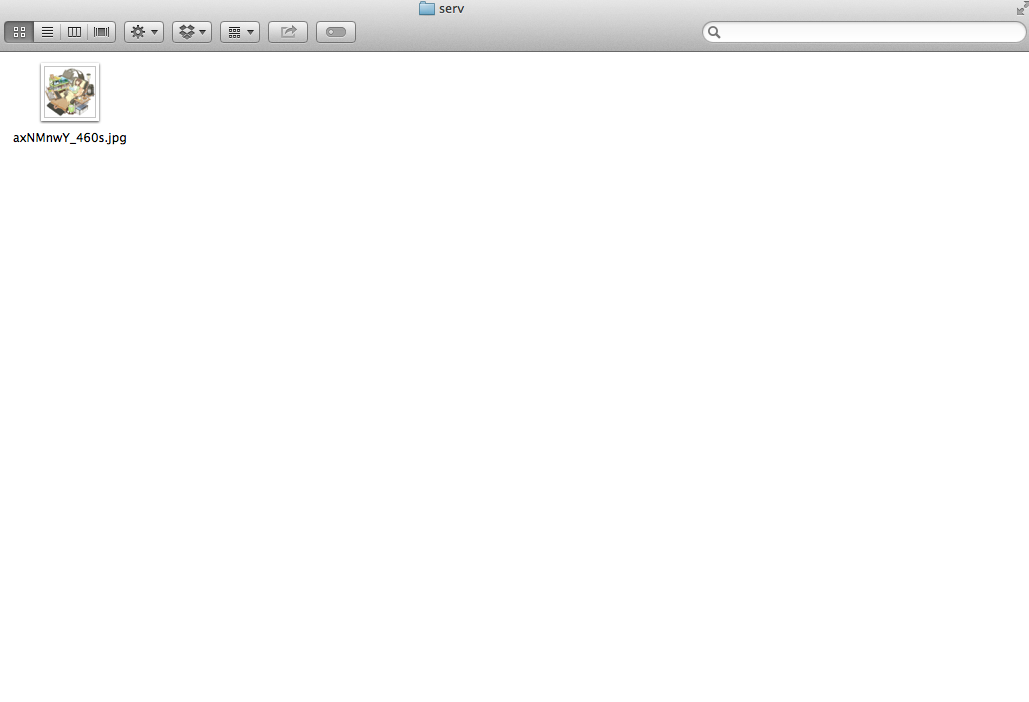
\includegraphics[scale=0.23]{anduvo.png}
		\caption*{¡Anduvo!}
	\end{figure}		
\end{frame}

\begin{frame}\frametitle{Sigamos probando}
	\begin{itemize}[<+->]
		\item Ahora sacale esto...
		\item ¿Sigue andando?
		\item Si, buenísimo, cambiale esto otro.
		\item Probalo de vuelta...
	\end{itemize}
\end{frame}


\begin{frame}\frametitle{Y cuando nos dimos cuenta...}
	\begin{figure}[htbp]
		\centering
		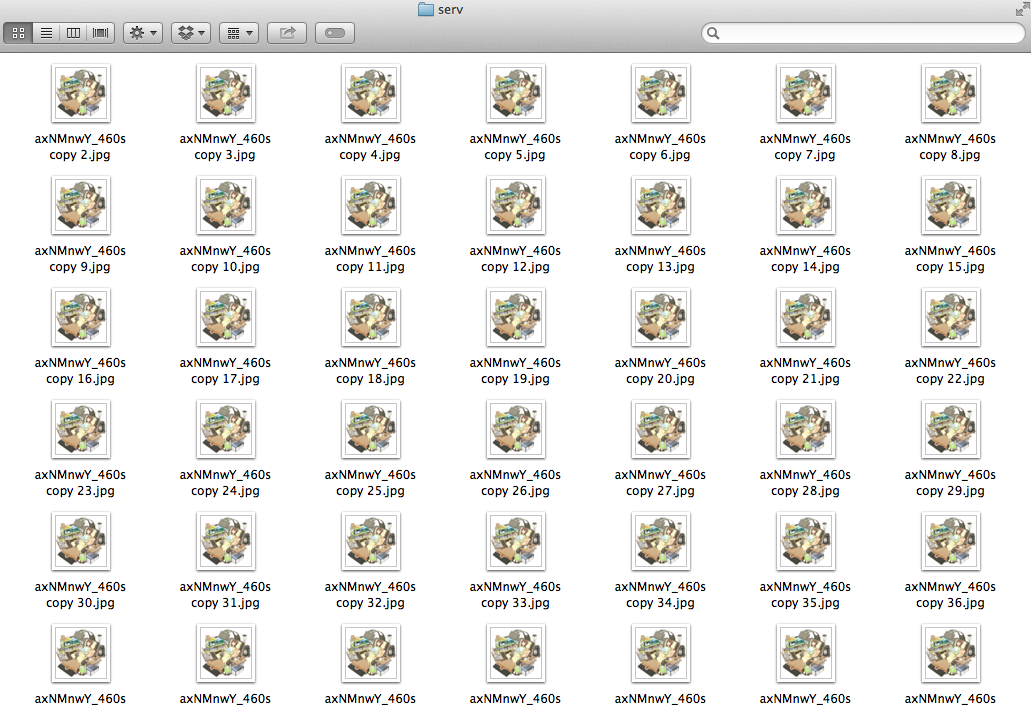
\includegraphics[scale=0.23]{muchasCopias.png}
		\caption*{¡Tenemos un problema Willy!}
	\end{figure}
\end{frame}

\begin{frame}\frametitle{A ver, a ver...}
	\begin{itemize}[<+->]
		\item Claramente esto no da.
		\item Dos problemas:
		\begin{enumerate}[<+->]
			\item Se nos guarda demasiadas veces cada foto.
			\begin{itemize}[<+->]
				\item No es tan grave, vamos a sobrevivir.
			\end{itemize}
			\item Estamos usando tráfico de red a lo loco al p...
			\item ...inútilmente.
			\begin{itemize}
				\item Esto no esá bueno.
			\end{itemize}
		\end{enumerate}
	\end{itemize}
\end{frame}

\begin{frame}\frametitle{sinRepetidos(miLista)}
	\begin{itemize}
		\item ¿Cómo sabemos qué imágenes ya se mandaron al server?
		\item Dos opciones:
		\begin{itemize}[<+->]
			\item Que el app guarde qué imágenes ya subió.
			\begin{itemize}[<+->]
				\item ¿Y si el usuario borra la data del app?
				\item ¿Y si el usuario se pone a ver la data del app?
				\item (¿Por qué este app está guardando una lista de mis imágenes?)
			\end{itemize}
		\end{itemize}
	\end{itemize}
\end{frame}

\begin{frame}\frametitle{Otra opción}
	\begin{itemize}[<+->]
		\item Mmm... el server sabe que fotos tiene.
		\item ¡Idea!
	\end{itemize}
\end{frame}

\begin{frame}\frametitle{Otra opción}
	\begin{itemize}
		\item Mmm... el server sabe que fotos tiene.
		\item ¡Idea!
	\end{itemize}
	\begin{figure}[htbp]
		\centering
		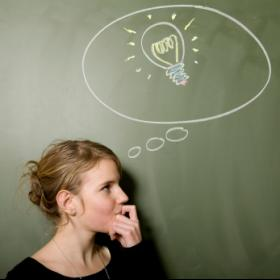
\includegraphics[scale=0.23]{idea.jpg}
		\caption*{(Vane no quiso posar)}
	\end{figure}
	\begin{itemize}[<+->]
		\item \textbf{¡Mandemos un \texttt{SHA-1} de la imágen y que el server nos diga si la tiene o no!}
	\end{itemize}
\end{frame}

\begin{frame}\frametitle{Probemos...}
	\begin{figure}[htbp]
		\centering
		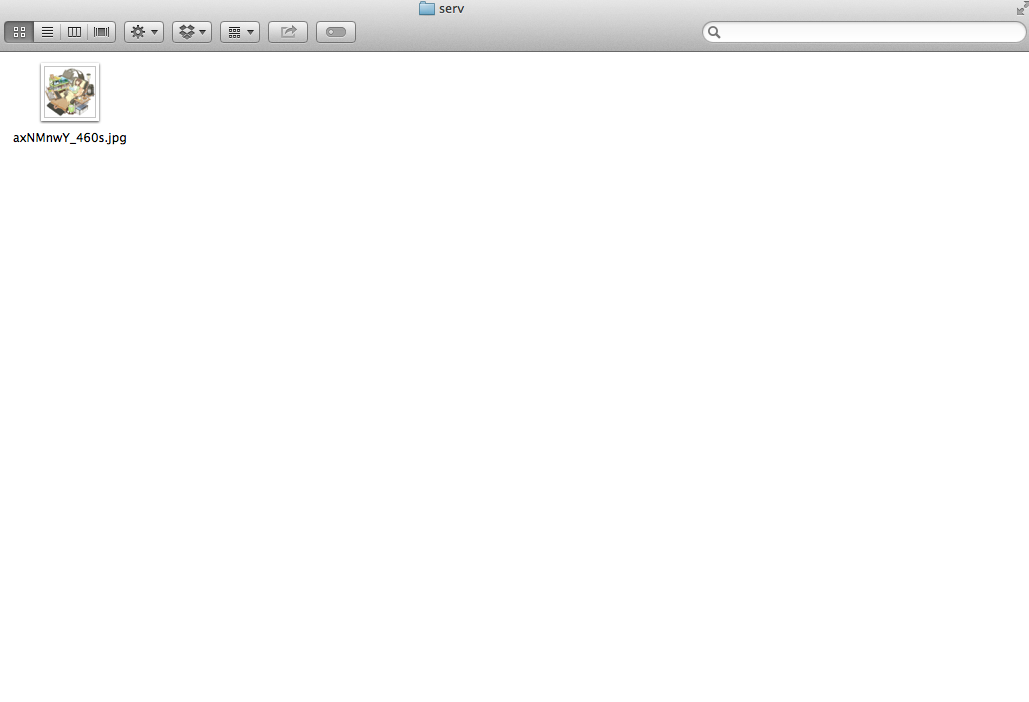
\includegraphics[scale=0.20]{anduvo.png}
		\caption*{(Nooo, no es la misma captura que antes)}
	\end{figure}
\end{frame}

\begin{frame}\frametitle{App andando}
	Genial, ya tenemos la aplicación andando!
	\begin{figure}[htbp]
		\centering
		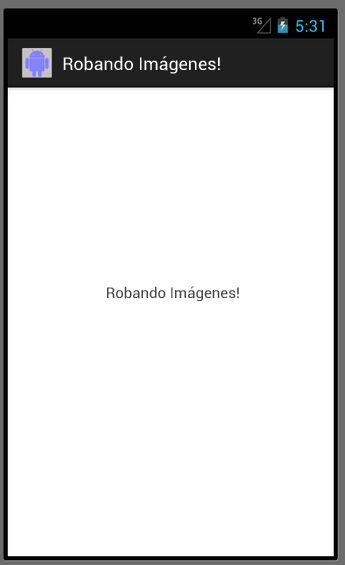
\includegraphics[scale=0.30]{appFea.png}
		% \caption*{(Nooo, no es la misma captura que antes)}
	\end{figure}
\end{frame}

\begin{frame}\frametitle{Estrategia de venta}
	\begin{itemize}[<+->]
		\item Después de pensarlo por horas....
		\item ...días...
		\item Se nos ocurrió que quizás...
		\item ...sólo quizas...
		\item ...la gente no quiera bajarse un app que lo único que tiene es un cartel que dice ``Robando fotos''.
	\end{itemize}
\end{frame}

\begin{frame}\frametitle{Estrategia de venta}
	\begin{itemize}[<+->]
		\item Necesitamos una \emph{fachada} para nuestro app roba fotos.
		\item Una fachada que verifique:
		\begin{itemize}
			\item Ser atractiva (sea por funcionalidad o aspecto visual).
			\item (Idealmente) Que justifique \textbf{un poco} los permisos que requiere el app.
			\item Por último...
			\item ...y más importante...
			\item ...que sea fácil y rápida de hacer.
		\end{itemize}
		\item Y así llegamos a....
	\end{itemize}
\end{frame}

\begin{frame}\frametitle{Destino Final}
	\begin{figure}[htbp]
		\centering
		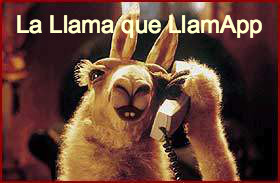
\includegraphics[scale=0.90]{llama.jpg}
		\caption*{(Marca Registrada)}
	\end{figure}
\end{frame}

\begin{frame}\frametitle{Mejoras}
	Una banda:
	\begin{itemize}[<+->]
		\item Hacer un solo post para las imagenes que tiene el servidor en vez de muchos.
		\item Funcionar en background.
		\item Guardar las imágenes en el servidor por \texttt{imei} (más ordenado).
		\item Encriptar las fotos que viajan por la red.
		\begin{itemize}[<+->]
			\item (No queremos darle 100 años de perdón a nadie).
		\end{itemize}
		\item Poder setear sonidos como \emph{ringtone}.
		\begin{itemize}
			\item Mejorar la Fachada en general.
		\end{itemize}
	\end{itemize}
\end{frame}

\section{Segunda parte: robando de todo}
\begin{frame}\frametitle{Ransomware}
	\begin{itemize}[<+->]
		\item Decidimos implementar un \emph{RAT} llamado \texttt{SuperSafeApp}.
	\end{itemize}
\end{frame}

\begin{frame}\frametitle{Mandando instrucciones}
	\begin{itemize}[<+->]
		\item El celular no tiene una ip fija a donde se le puedan mandar mensajes...
		\item ¿Cómo mandamos instrucciones al celular?
		\item Varias opciones:
		\begin{itemize}[<+->]
			\item Usar algún servicio como no-ip y levantar un servidor en el celular
			\begin{itemize}[<+->]
				\item (¿se puede eso?)
				\item Nah, mucho laburo
			\end{itemize}
			\item POST
			\begin{itemize}[<+->]
				\item Hacer polling al server
				\item (PUAJJJ)
			\end{itemize}
			\item Push
			\begin{itemize}[<+->]
				\item Hay que registrarse... fiaca.
			\end{itemize}
		\end{itemize}
	\end{itemize}
\end{frame}

\begin{frame}\frametitle{No hay ``cosa'' que les venga bien}
	\begin{itemize}[<+->]
		\item ¿Y entonces?
		\item Queremos una forma más fácil...
		\item ...si tan solo hubiera una forma que se usara diariamente por millones de personas para mandarle un mensaje de texto corto a un celular....
		\item SMS!
	\end{itemize}
\end{frame}

\begin{frame}\frametitle{Comandos}
	\begin{itemize}[<+->]
		\item Los comandos recibidos por sms tienen el formato:
	\end{itemize}
	\begin{center}
		\texttt{<<!COMANDO>>(parametro1,parametro2,....)}
	\end{center}
\end{frame}

\begin{frame}\frametitle{Comandos aceptados}
	\begin{itemize}
		\item Los comandos que acepta el RAT son:
		\begin{itemize}
			\item $<<!VIBRATE>>$
			\item $<<!CONTACTS>>$
			\item $<<!RANSOM>>(archivo)$
			\item $<<!PHOTO>>$
			\item $<<!SENDSMS>>(destino,mensaje)$
			\item $<<!LOCATION>>$
			\item $<<!CALLLOG>>$
		\end{itemize}
	\end{itemize}
\end{frame}

\begin{frame}\frametitle{Pidiendo rescate}
	\begin{itemize}[<+->]
		\item Para evitar que el usuario sospeche, \texttt{SuperSafeApp} funciona coordinado con otra aplicación (\texttt{Ransomwarer}) para encriptar los archivos. 
		\item Ambas aplicaciones están firmadas con la misma clave, con lo que pueden intercambiar información.
	\end{itemize}
\end{frame}

\begin{frame}\frametitle{Mejoras}
	También son muchas:
	\begin{itemize}[<+->]
		\item $<<!RANSOM>>(archivo, cifrar|descifrar)$
		\item $<<!RANSOM>>(directorio, cifrar|descifrar)$
		\item $<<!RANSOM>>(\_\_ALL\_\_, cifrar|descrifrar)$
		\item $<<!SENDSMS>>(\_\_ALL\_\_, mensaje)$
		\begin{itemize}
			\item Aguante \emph{spammear} gente.
		\end{itemize}
		\item Funcionar en background.
		\item Seleccionar Wifi - 3G.
		\item Partirlo en varias aplicaciones firmadas con la misma clave...
		\item ...y venderlo como ``Pack de seguridad''.
	\end{itemize}	
\end{frame}

\end{document}
